\documentclass[12pt]{report}
\usepackage[utf8]{inputenc}
\usepackage[russian]{babel}
%\usepackage[14pt]{extsizes}
\usepackage{listings}
\usepackage{graphicx}
\usepackage{amsmath,amsfonts,amssymb,amsthm,mathtools} 
\usepackage{pgfplots}
\usepackage{filecontents}
\usepackage{indentfirst}
\usepackage{eucal}
\usepackage{amsmath}
\usepackage{enumitem}
\frenchspacing

\usepackage{indentfirst} % Красная строка


%\usetikzlibrary{datavisualization}
%\usetikzlibrary{datavisualization.formats.functions}

\usepackage{amsmath}




% Для листинга кода:
\lstset{ %
language=haskell,                 % выбор языка для подсветки (здесь это С)
basicstyle=\small\sffamily, % размер и начертание шрифта для подсветки кода
numbers=left,               % где поставить нумерацию строк (слева\справа)
numberstyle=\tiny,           % размер шрифта для номеров строк
stepnumber=1,                   % размер шага между двумя номерами строк
numbersep=5pt,                % как далеко отстоят номера строк от подсвечиваемого кода
showspaces=false,            % показывать или нет пробелы специальными отступами
showstringspaces=false,      % показывать или нет пробелы в строках
showtabs=false,             % показывать или нет табуляцию в строках
frame=single,              % рисовать рамку вокруг кода
tabsize=2,                 % размер табуляции по умолчанию равен 2 пробелам
captionpos=t,              % позиция заголовка вверху [t] или внизу [b] 
breaklines=true,           % автоматически переносить строки (да\нет)
breakatwhitespace=false, % переносить строки только если есть пробел
escapeinside={\#*}{*)}   % если нужно добавить комментарии в коде
}

\usepackage[left=2cm,right=2cm, top=2cm,bottom=2cm,bindingoffset=0cm]{geometry}
% Для измененных титулов глав:
\usepackage{titlesec, blindtext, color} % подключаем нужные пакеты
\definecolor{gray75}{gray}{0.75} % определяем цвет
\newcommand{\hsp}{\hspace{20pt}} % длина линии в 20pt
% titleformat определяет стиль
\titleformat{\chapter}[hang]{\Huge\bfseries}{\thechapter\hsp\textcolor{gray75}{|}\hsp}{0pt}{\Huge\bfseries}


% plot
\usepackage{pgfplots}
\usepackage{filecontents}
\usetikzlibrary{datavisualization}
\usetikzlibrary{datavisualization.formats.functions}

\begin{document}
\setcounter{page}{2}
\tableofcontents

\newpage
\chapter*{Введение}
\addcontentsline{toc}{chapter}{Введение}
RISC-V является открытым современным набором команд, который может использоваться для построения как микроконтроллеров, так и высокопроизводительных микропроцессоров. В связи с такой широкой областью применения в систему команд введена вариативность. Таким образом, термин RISC-V фактически является названием для семейства различных систем команд, которые строятся вокруг базового набора команд, путем внесения в него различных расширений.

\textbf{Цель работы}: ознакомление с принципами функционирования, построения и особенностями архитектуры суперскалярных конвейерных микропроцессоров, а также знакомство с принципами проектирования и верификации сложных цифровых устройств с использованием языка описания аппаратуры SystemVerilog и ПЛИС.
Для достижения данной цели необходимо выполнить следующие задачи:
\begin{itemize}
    \item ознакомиться с набором команд RV32I;
    \item ознакомиться с основными принципами работы ядра Taiga: изучить операции, выполняемые на каждой стадии обработки команд;
    \item на основе полученных знаний проанализировать ход выполнения программы и оптимизировать ее; 
\end{itemize}

В настоящей лабораторной работе используется синтезируемое описание микропроцессорного ядра Taiga, реализующего систему команд RV32I семейства RISC-V. Данное описание выполнено на языке описания аппаратуры SystemVerilog.

Все задания выполняются в соответствии с вариантом №4.

\chapter{Задание № 1}
\section{Текст программы по индивидуальному варианту}
Текст программы по индивидуальному варианту приведён на листинге \ref{programText}
\begin{lstlisting}[label=programText,caption=Текст программы по индивидуальному варианту]
        .section .text
        .globl _start;
        len = 8
        enroll = 1 
        elem_sz = 4 

_start:
        la x1, _x                       // into x1 beginning of mas
        addi x20, x1, elem_sz*(len-1)   // x20 = x1 + (len - 1) * size
lp:
        lw x2, 0(x1)                    // x2 = x1[0]
        addi x1, x1, elem_sz*enroll #!  // x1 += elem_sz;
        add x31, x31, x2                // x31 += x2;
        bne x1, x20, lp                 // if (x1 != x20) goto lp;
        addi x31, x31, 1                // x31 += 1
lp2: j lp2

        .section .data
_x:     .4byte 0x1
        .4byte 0x2
        .4byte 0x3
        .4byte 0x4
        .4byte 0x5
        .4byte 0x6
        .4byte 0x7
        .4byte 0x8
\end{lstlisting}

Анализируя исходный текст программы, было выяснено, что в регистре x31 в конце выполнения программы должно содержаться значение:
\begin{displaymath}
x31 = \sum\limits_{i=1}^7{i} + 1 = 29.
\end{displaymath}

\section{Дизассемблерный листинг кода программы}
В результате выполнения компиляции был создан файл с расширением .hex, хранящий содержимое памяти команд и данных. В окне терминала отобразился дизассемблерный листинг, который приведён в листинге \ref{disasmListing}.

\begin{lstlisting}[label=disasmListing,caption=Дизассемблерный листинг кода программы]
SYMBOL TABLE:
80000000 l    d  .text  00000000 .text
80000024 l    d  .data  00000000 .data
00000000 l    df *ABS*  00000000 main.o
00000008 l       *ABS*  00000000 len
00000001 l       *ABS*  00000000 enroll
00000004 l       *ABS*  00000000 elem_sz
80000024 l       .data  00000000 _x
8000000c l       .text  00000000 lp
80000020 l       .text  00000000 lp2
80000000 g       .text  00000000 _start
80000044 g       .data  00000000 _end

Disassembly of section .text:

80000000 <_start>:
80000000:       00000097                auipc   x1,0x0
80000004:       02408093                addi    x1,x1,36 # 80000024 <_x>
80000008:       01c08a13                addi    x20,x1,28

8000000c <lp>:
8000000c:       0000a103                lw      x2,0(x1)
80000010:       00408093                addi    x1,x1,4
80000014:       002f8fb3                add     x31,x31,x2
80000018:       ff409ae3                bne     x1,x20,8000000c <lp>
8000001c:       001f8f93                addi    x31,x31,1

80000020 <lp2>:
80000020:       0000006f                jal     x0,80000020 <lp2>

Disassembly of section .data:

80000024 <_x>:
80000024:       0001                    c.addi  x0,0
80000026:       0000                    unimp
80000028:       0002                    0x2
8000002a:       0000                    unimp
8000002c:       00000003                lb      x0,0(x0) # 0 <enroll-0x1>
80000030:       0004                    c.addi4spn      x9,x2,0
80000032:       0000                    unimp
80000034:       0005                    c.addi  x0,1
80000036:       0000                    unimp
80000038:       0006                    0x6
8000003a:       0000                    unimp
8000003c:       00000007                0x7
80000040:       0008                    c.addi4spn      x10,x2,0

\end{lstlisting}

\newpage
\chapter{Задание №2}
\section{Выполнение}
В результате симуляции, был получен снимок экрана, содержащий временную диаграмму выполнения стадий выборки и диспетчеризации команды с адресом 80000018 (1 итерация). Снимок экрана приведён на рисунке \ref{fetchDispatch80000018}.

\begin{figure}[h!p]
	\centering
	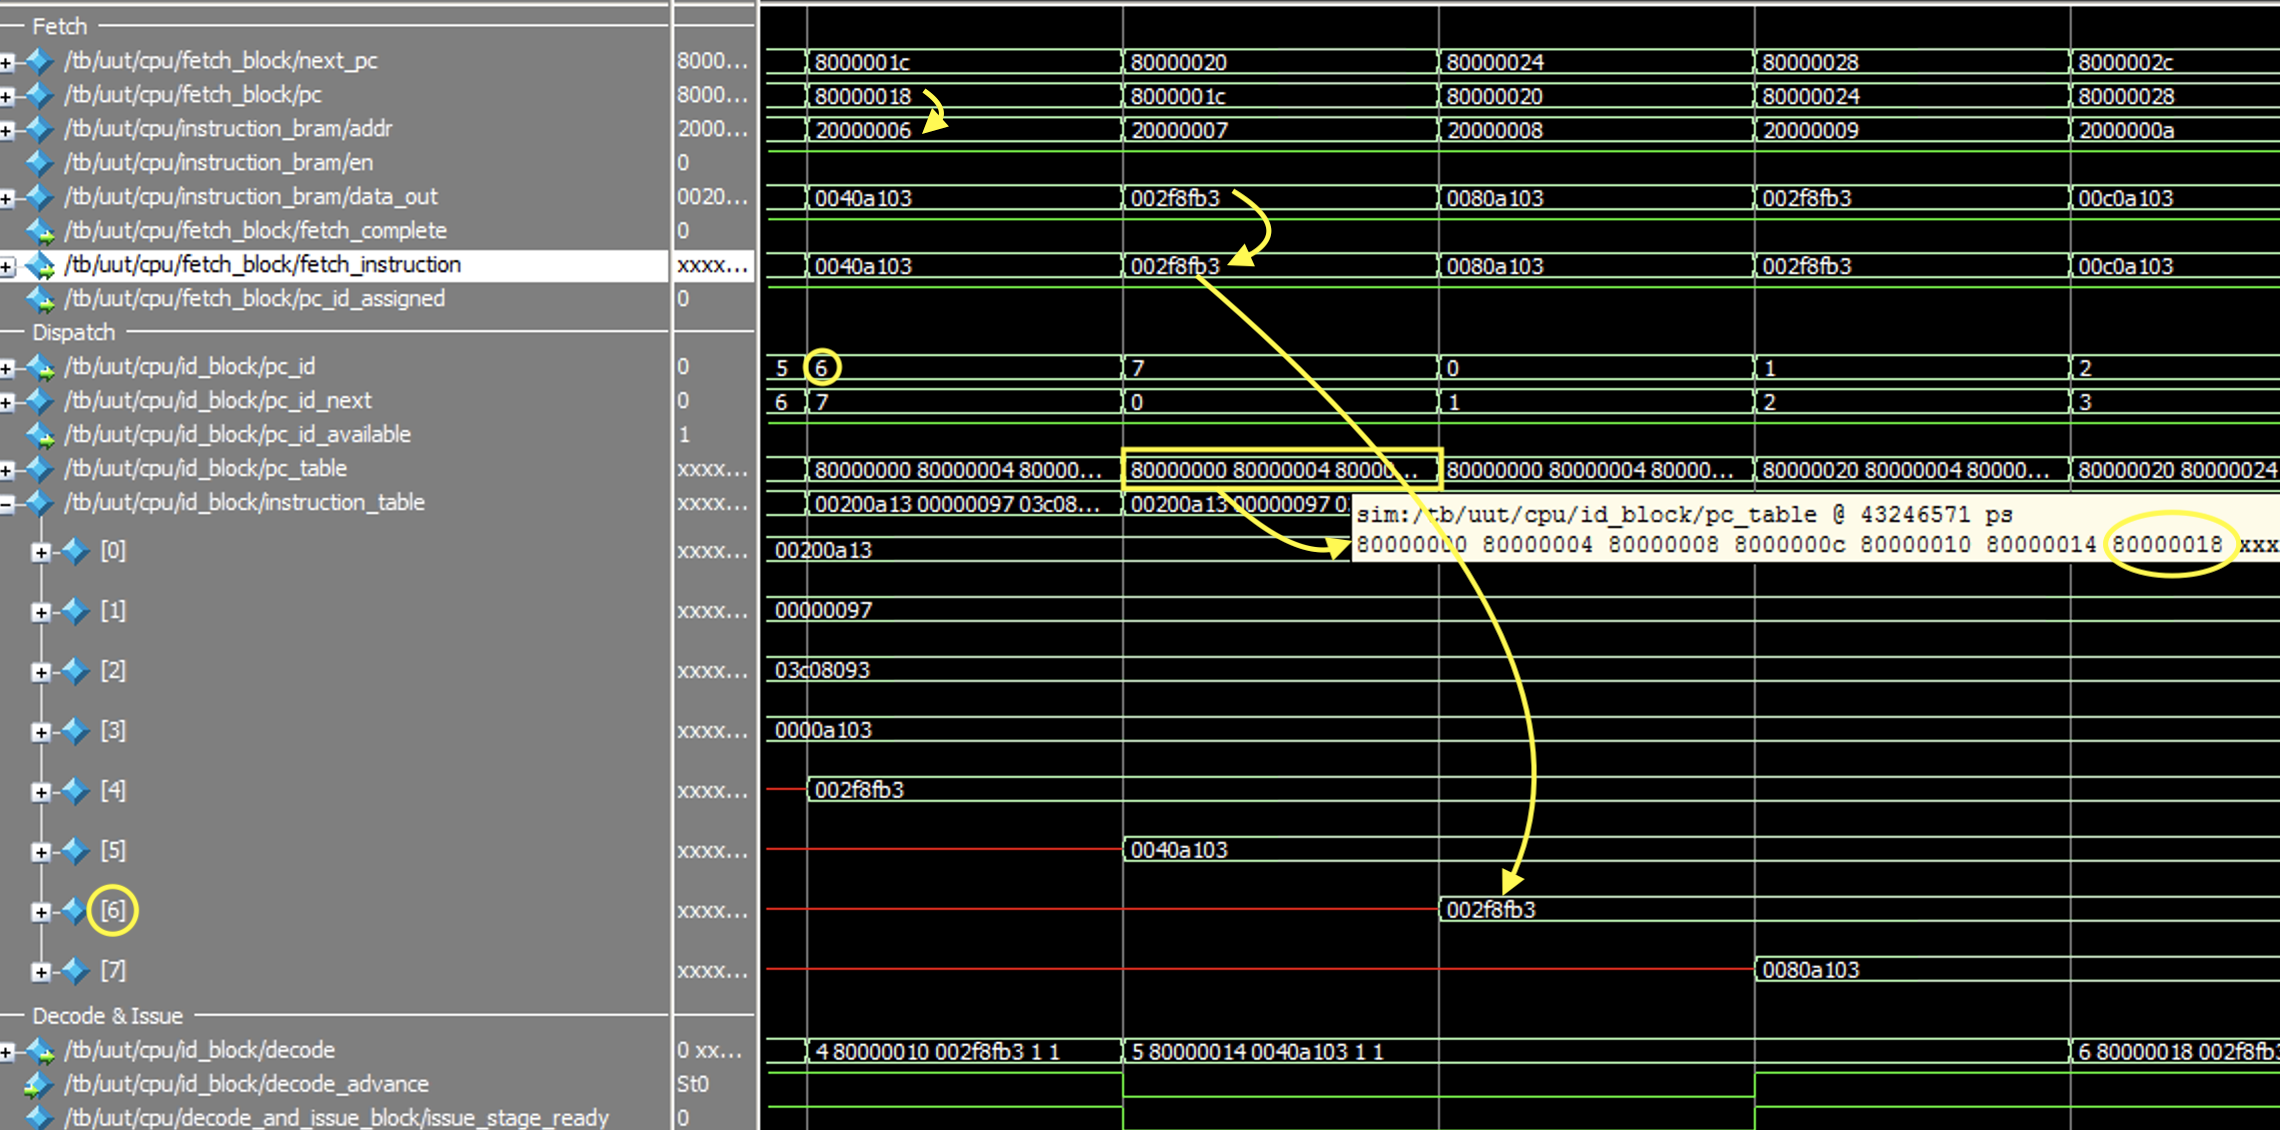
\includegraphics[width = \linewidth]{fetchDispatch80000018.png}
	\caption{Временная диаграмма выполнения стадий выборки и диспетчеризации команды с адресом 80000018 (1 итерация)}
	\label{fetchDispatch80000018}
\end{figure}
Рассмотрим происходящее на рисунке \ref{fetchDispatch80000018}. Будем называть первым тактом самый левый такт на рисунке.
\begin{itemize}
    \item На 1 такте \verb|pc| = 80000018. Этот адрес выставляется на ША памяти команд (причём адрес получается с помощью деления на 4, так как память в RISC-V адресуется в байтах, а память команд адресуется блоками по 4 байта). Таким образом, \verb|instruction_bram/addr| = 20000006. Идентификатор команды (\verb|pc_id|) присваивается в момент начала выборки, то есть одновременно с выставлением адреса команды на ША памяти команд. Кроме того, по фронту \verb|clk|, завершающему такт адрес команды(то есть, значение регистра \verb|pc| на момент выборки) записывается в таблицу \verb|pc_table| по присвоенному идентификатору.  
    \item На 2 такте память команд выдает данные (то есть, код команды), прочитанные по адресу, который был выставлен на ША в предыдущем такте (сигнал \verb|data_out|). Блок выборки выдает эти данные на линию \verb|fetch_instruction|. Устанавливается сигнал \verb|fetch_complete|, подтверждающий выборку и наличие кода команды на линии \verb|fetch_ins|-\verb|truction|. В \verb|pc| записывается адрес следующей команды.
    \item На 3 такте код команды записывается в таблицу \verb|instruction_table| по идентификатору, который был присвоен ранее.
\end{itemize}

\chapter{Задание №3}
\section{Выполнение}
После того, как на выходе блока управления метаинформацией сформирован пакет данных, описывающих очередную инструкцию (то есть, поле decode.valid принимает значение 1) начинается этап
декодирования этой инструкции и планирования ее на выполнение. Данный этап выполняется блоком декодирования и планирования на выполнение.

В результате симуляции, был получен снимок экрана, содержащий временную диаграмму выполнения стадии декодирования и планирования на выполнение команды с адресом 80000024 (1 итерация). Снимок экрана приведён на рисунке \ref{decode80000024}.

\begin{figure}[h!p]
	\centering
	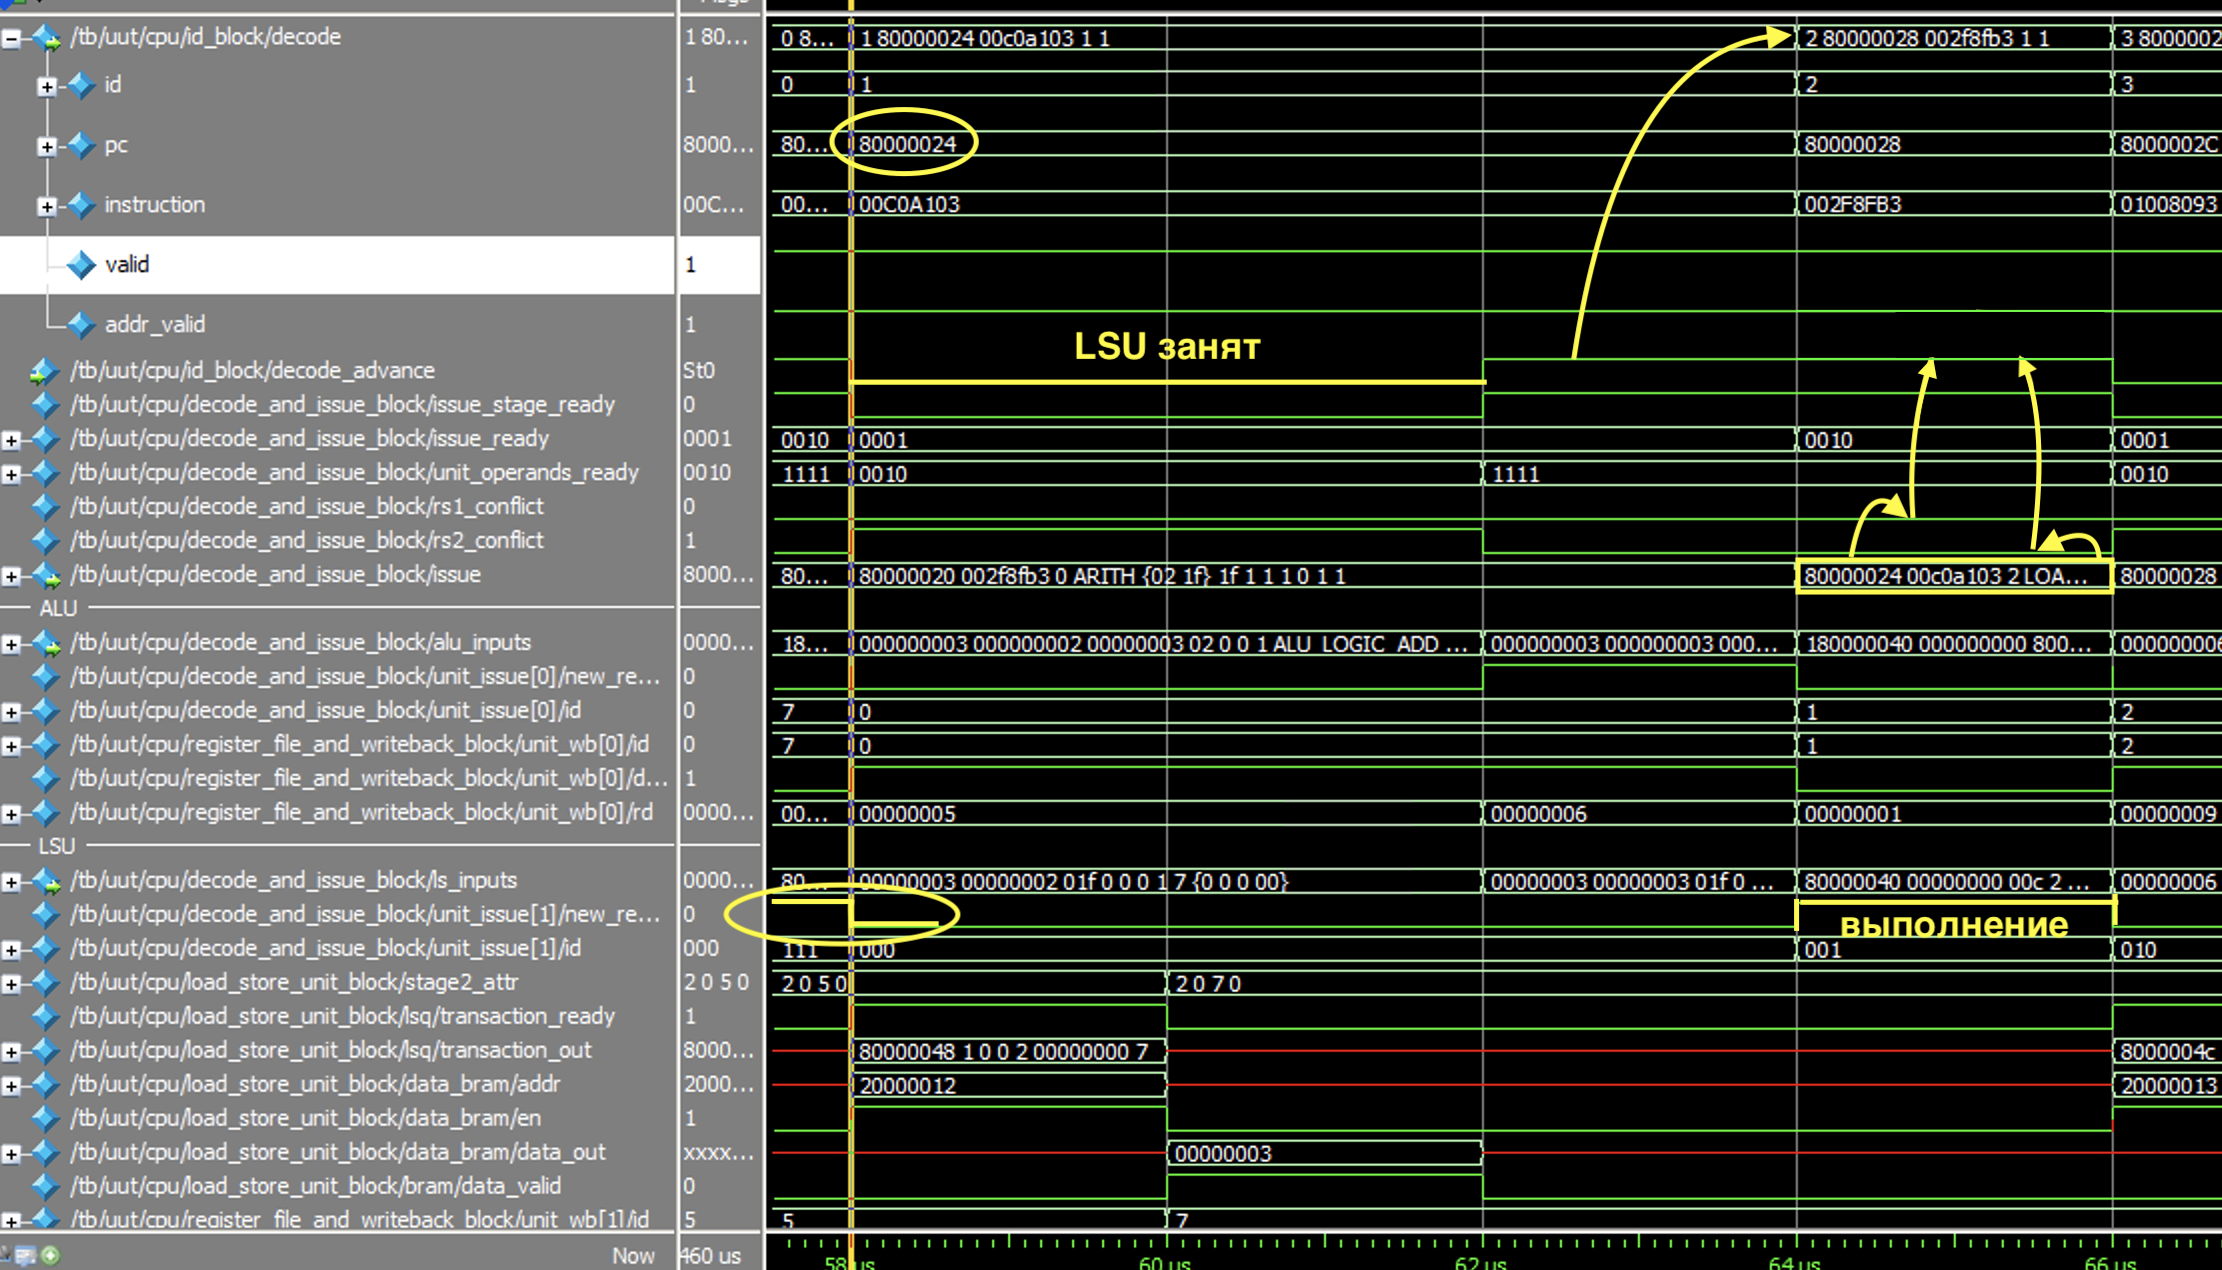
\includegraphics[width = \linewidth]{decode80000024.png}
	\caption{Временная диаграмма выполнения стадии декодирования и планирования на выполнение команды с адресом 80000024 (1 итерация)}
	\label{decode80000024}
\end{figure}

Рассмотрим происходящее на рисунке \ref{decode80000024}. Будем называть первым тактом самый левый такт на рисунке.
\begin{itemize}
    \item В такте, предшествующем первому, происходит диспетчеризация команды с id=1. В такте 1 она поступает на вход блока декодирования (это видно по тому признаку, что сигнал decode.valid установлен).
    \item В такте 1 происходит декодирование команды. Команда не может быть запланирована на выполнение, так как занято устройство LSU (блок управления памятью, выполняющий команду), поэтому проходит 2 такта ожидания. При освобождении блока управления памятью устанавливается сигнал \verb|decode_advance| для передачи блоку управления метаинформацией указания выдать очередную команду для декодирования в следующем такте.
    \item В начале такта 4 выдаются сигналы для исполнительных блоков. На основании сигнала \verb|issue| формируются сигналы \verb|rs1_conflict|, \verb|rs2_conflict| равные 0, так как конфликта по регистрам нет. Отсутствие конфликта дает возможность точно выполнить данную команду в этом такте, соответственно сигнал \verb|decode_advance| должен быть установлен в 1.
\end{itemize}

 \chapter{Задание №4}
 \section{Выполнение}
После того, как команда запланирована для выполнения и нет конфликта по регистрам, начинается этап выполнения команды каким-либо исполнительным блоком. Однако, в начале этапа выполнения происходит чтение исходных регистров команды, информация о которых содержится в сигнале issue. Чтение регистрового файла выполняется комбинационно, то есть, данные на выходе регистрового файла выдаются в том же такте, что и сигнал issue.

В результате симуляции, был получен снимок экрана, содержащий временную диаграмму выполнения стадии выполнения команды с адресом 8000000c (1 итерация). Снимок экрана приведён на рисунке \ref{lsu8000000c}.

\begin{figure}[h!p]
	\centering
	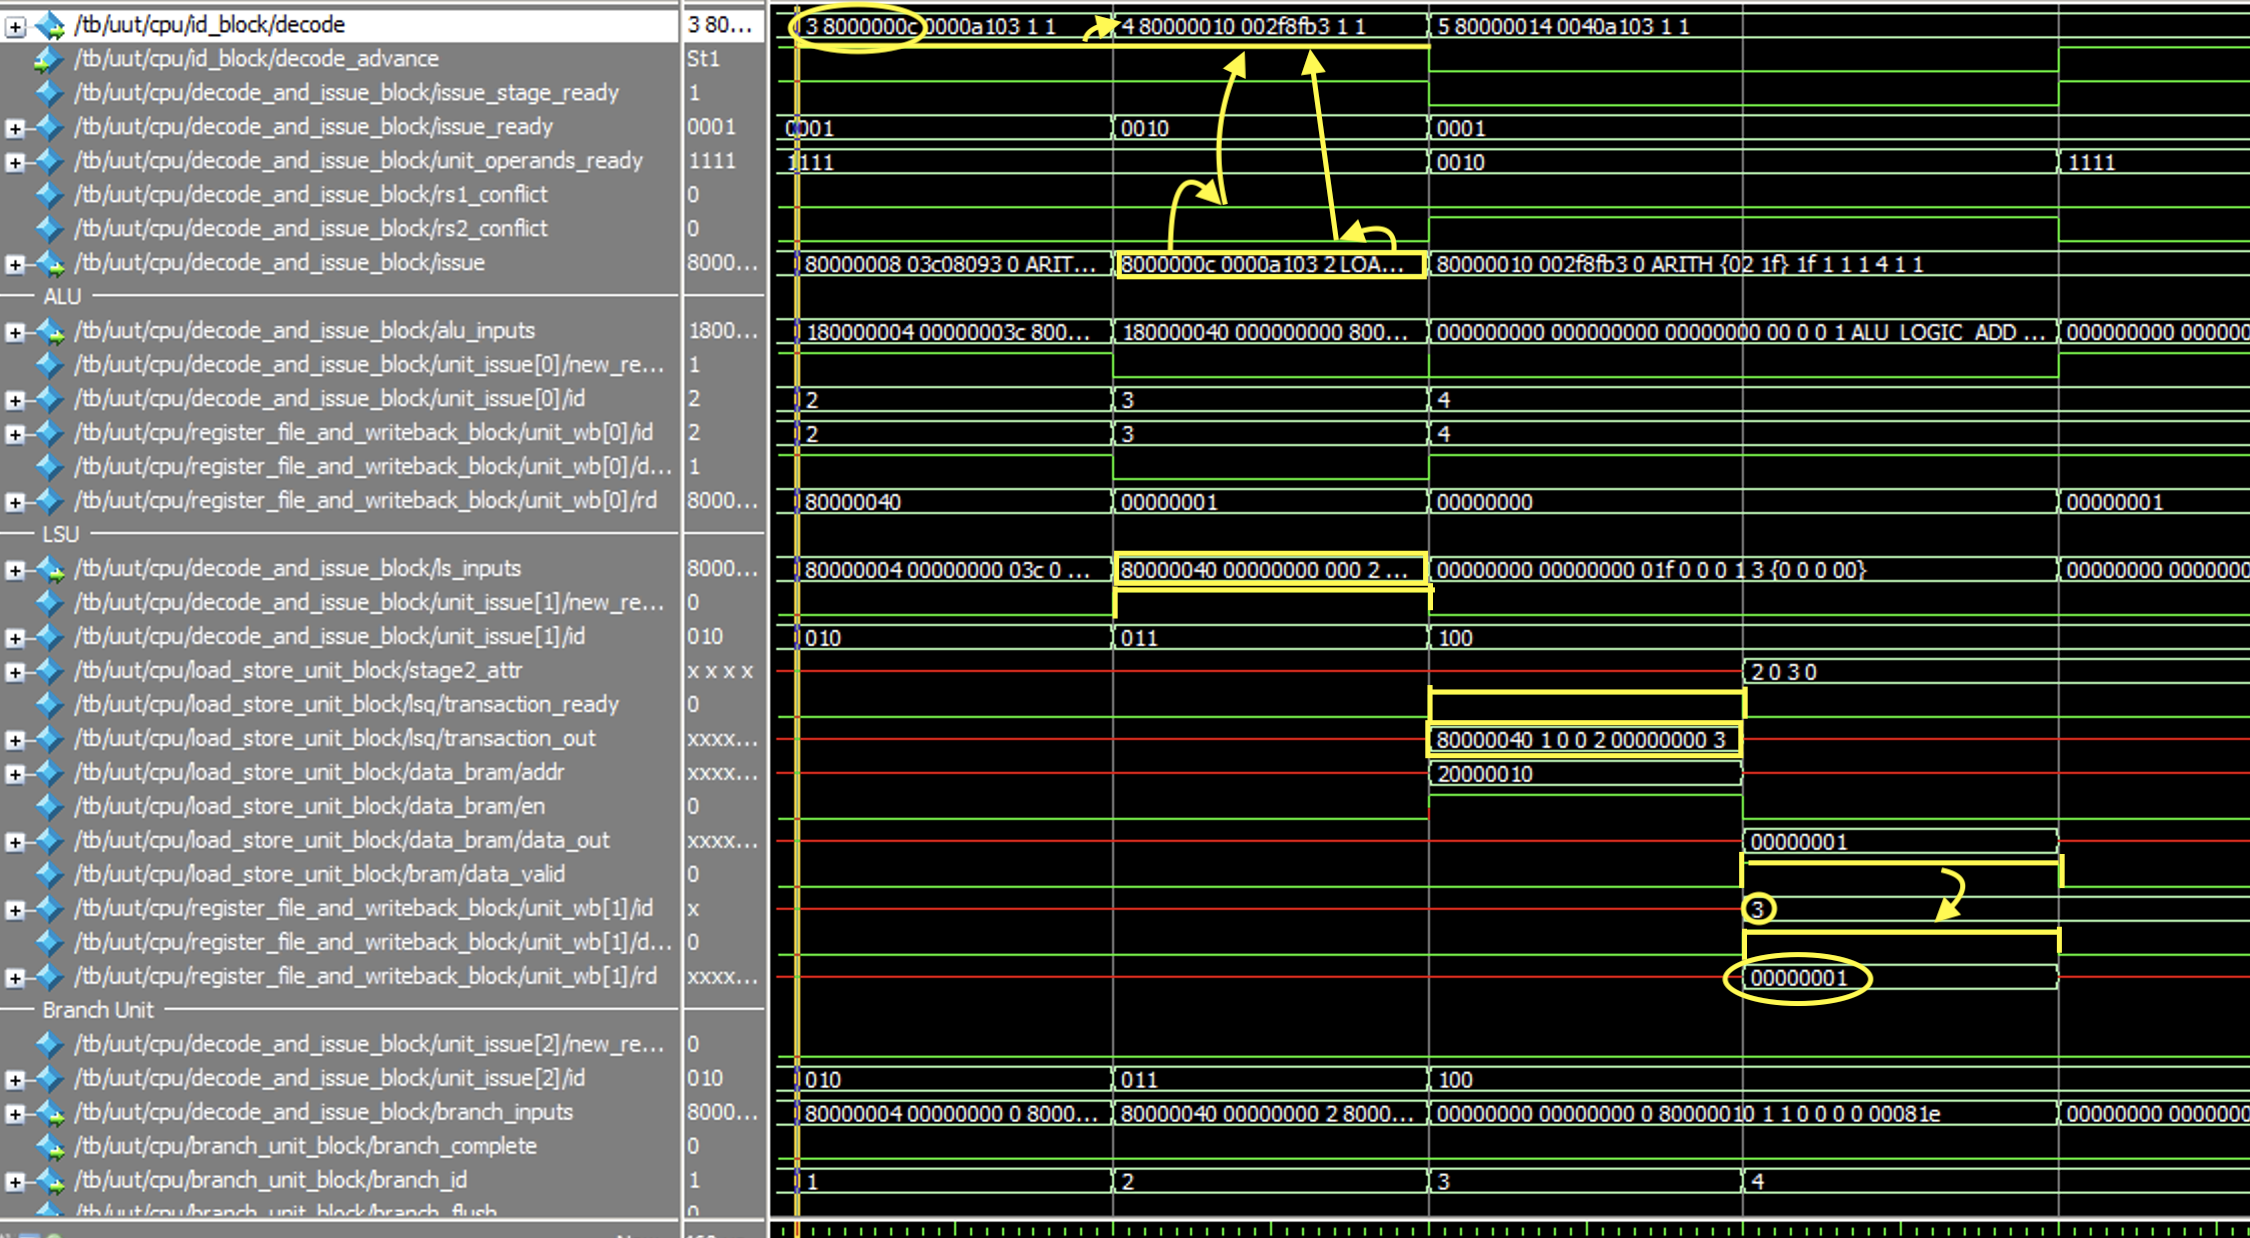
\includegraphics[width = \linewidth]{lsu8000000c.png}
	\caption{Временная диаграмма выполнения стадии декодирования и планирования на выполнение команды с адресом 8000000с (1 итерация)}
	\label{lsu8000000c}
\end{figure}

Рассмотрим происходящее на рисунке \ref{lsu8000000c}. Видно, что команда будет обработана блоком обращения к памяти.
\begin{itemize}
\item В момент планирования на выполнение новой команды (то есть, в момент выставления сигнала \verb|unit_issue[1].new_request|) происходит формирование на основе сигнала \verb|ls_inputs| атрибутов транзакции доступа к памяти (адрес, тип, размер и пр.) и их запись в очередь транзакций.
\item В следующем такте характеристики транзакции становятся доступны на выходе очереди транзакций (сигнал \verb|transaction_out|), что подтверждается сигналом \verb|transaction_ready|. Выполняется дешифрирование адреса и определение вида памяти к которой происходит доступ. Готовность памяти данных (в нашем случае, готовность памяти имеется всегда, так как время доступа к памяти всегда составляется 1 такт) дает возможность сформировать запрос к памяти, то есть выставить на ША адрес, соответствующий характеристикам транзакции. Адрес формируется комбинационно. Так как блок рассчитан на работу с памятью с неизвестной заранее задержкой, то характеристики запроса к памяти записываются в очередь запросов к памяти.
\item В следующем такте память данных выставляет на ШД прочитанные данные (сигнал \verb|data_out_b|) и сигнал готовности данных \verb|data_valid|. Блок фиксирует выполнение команды выставлением сигнала \verb|unit_wb[1].done| (формируется комбинационно по сигналу \verb|data_valid|), \verb|unit_wb[1].id| (берется из выхода очереди запросов к памяти) и \verb|unit_wb[1].rd| (берется с ШД памяти данных). В этом же такте происходит запись в целевой регистр. 
\end{itemize}

Таким образом видно, что выполнение команды доступа к памяти занимает минимум 3 такта.

\chapter{Задание №5}
В заданиях 2-4 симуляция проводилась на программе из примера. В задании №5 симуляция проводится на программе из индивидуального варианта, которая описана в 1 задании. 

\section{Сравнение полученного теоретически значения регистра x31 и полученного в результате симуляции}
Для проверки сравним значение регистра x31, вычисленного теоретически, с полученным в результате симуляции. Теоретически было получено значение 29. Результат симуляции представлен на рисунке \ref{x31check}. Видим, что значения совпадают, так как ${1D}_{16} = {29}_{10}$

\begin{figure}[h!p]
	\centering
	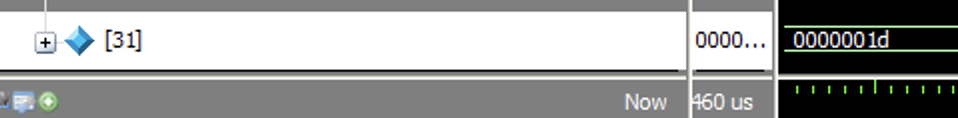
\includegraphics[width = \linewidth]{x31check.png}
	\caption{Значение регистра x31, полученное в результате симуляции}
	\label{x31check}
\end{figure}

\section{Временные диаграммы сигналов, соответствующих всем стадиям выполнения команды 80000010}
В тексте программы \ref{programText} символом \verb|#!| обозначена команда \verb|addi| \verb|x1|, \verb|x1|, \verb|elem_sz| * \verb|enroll|. Из дизассемблерного листинга кода программы \ref{disasmListing} очевидно, что эта команда имеет адрес \verb|80000010|.

На рисунках \ref{80000010_01} и \ref{80000010_02} приведены временные диаграммы сигналов, соответствующих всем стадиям выполнения команды с адресом 80000010.
\begin{figure}[h!p]
	\centering
	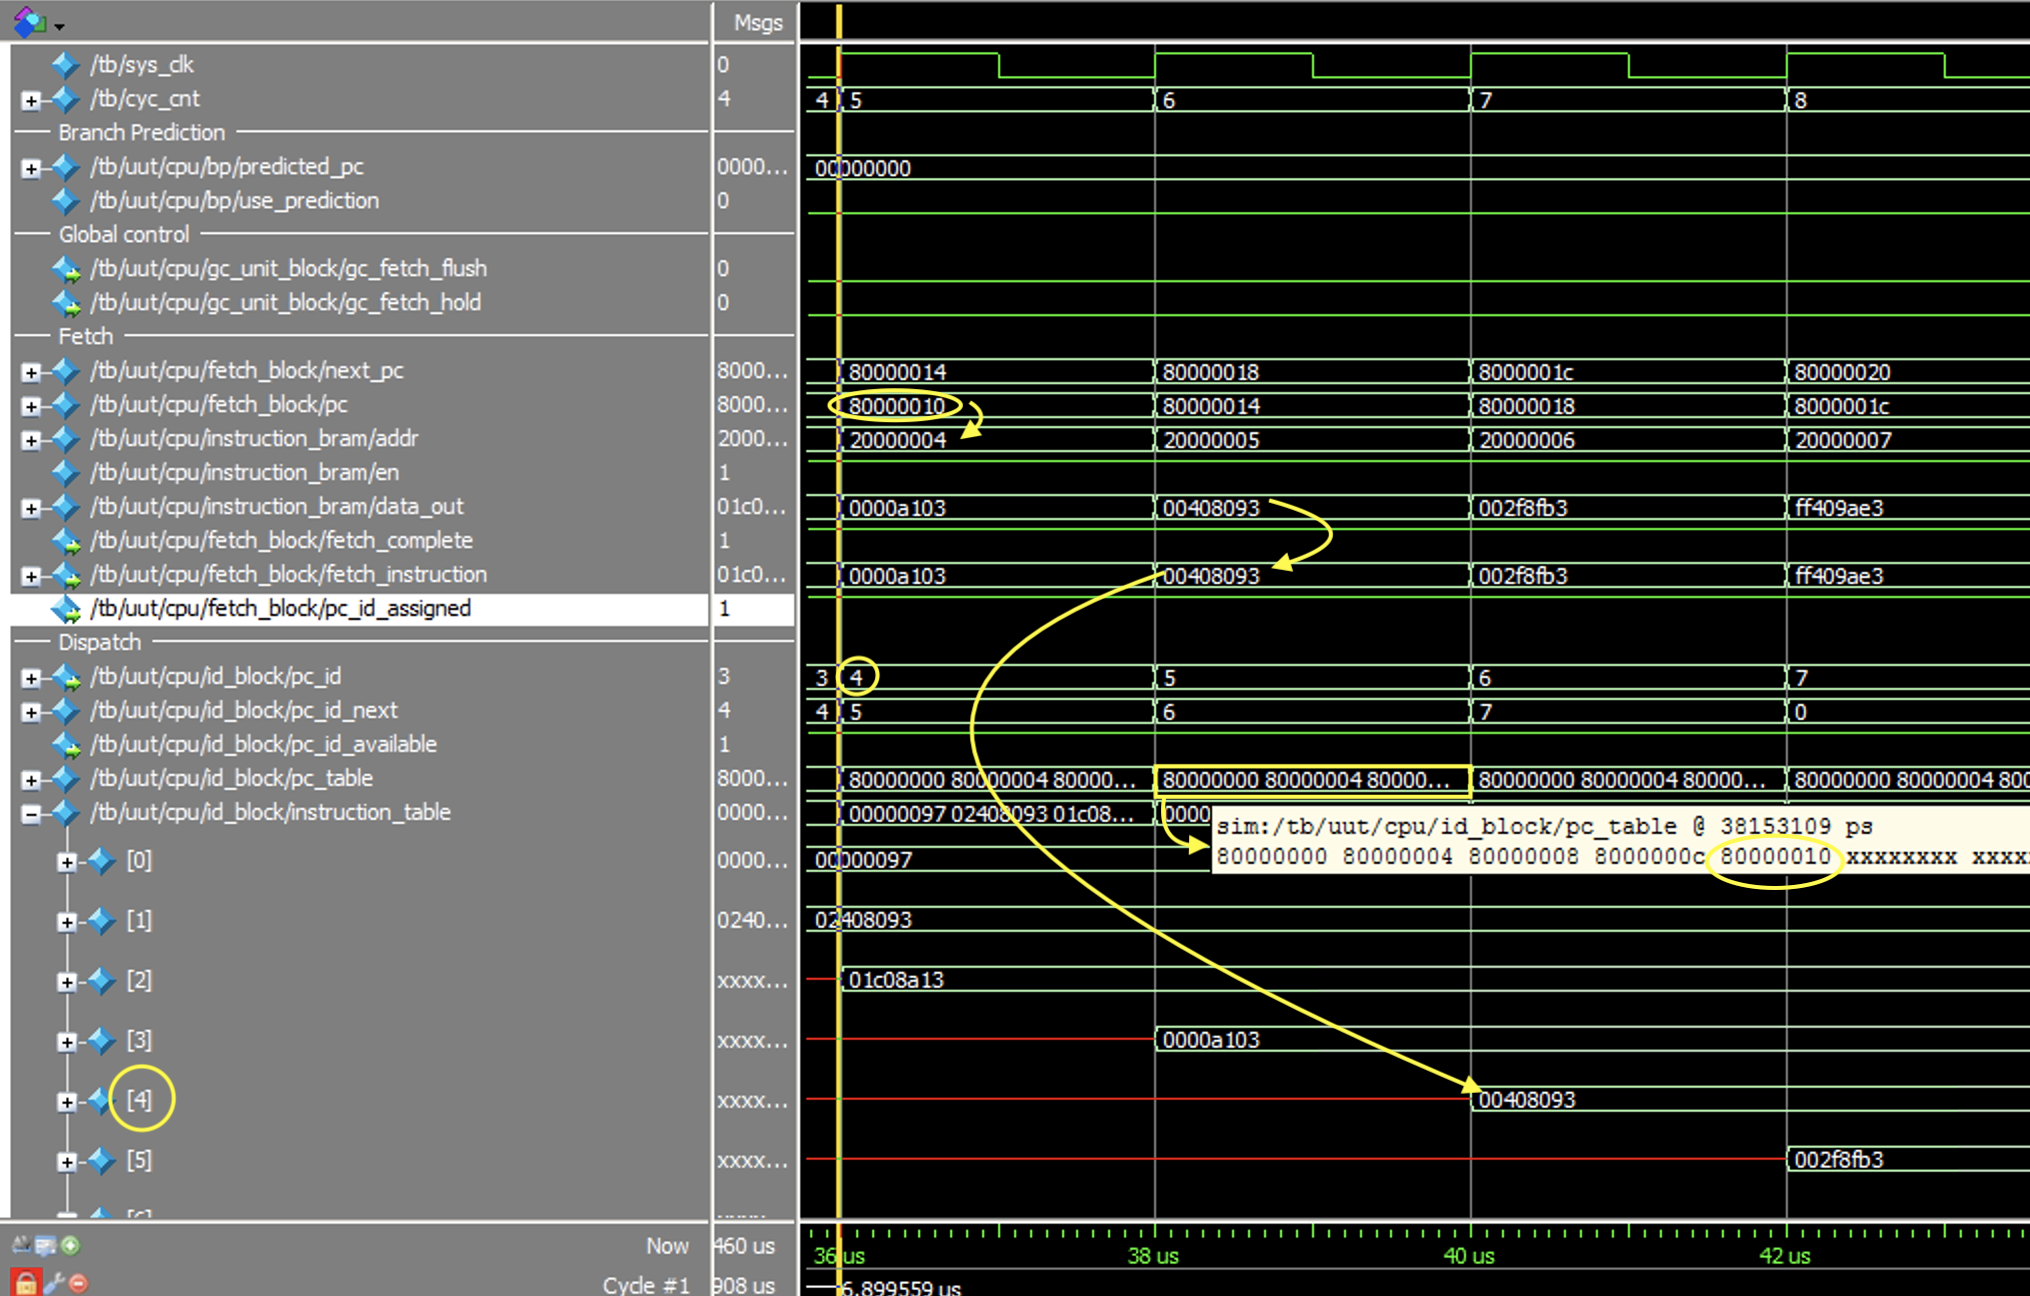
\includegraphics[width = \linewidth]{80000010_01.png}
	\caption{Временная диаграмма выполнения стадий выборки и диспетчеризации команды с адресом 80000010}
	\label{80000010_01}
\end{figure}

\begin{figure}[h!p]
	\centering
	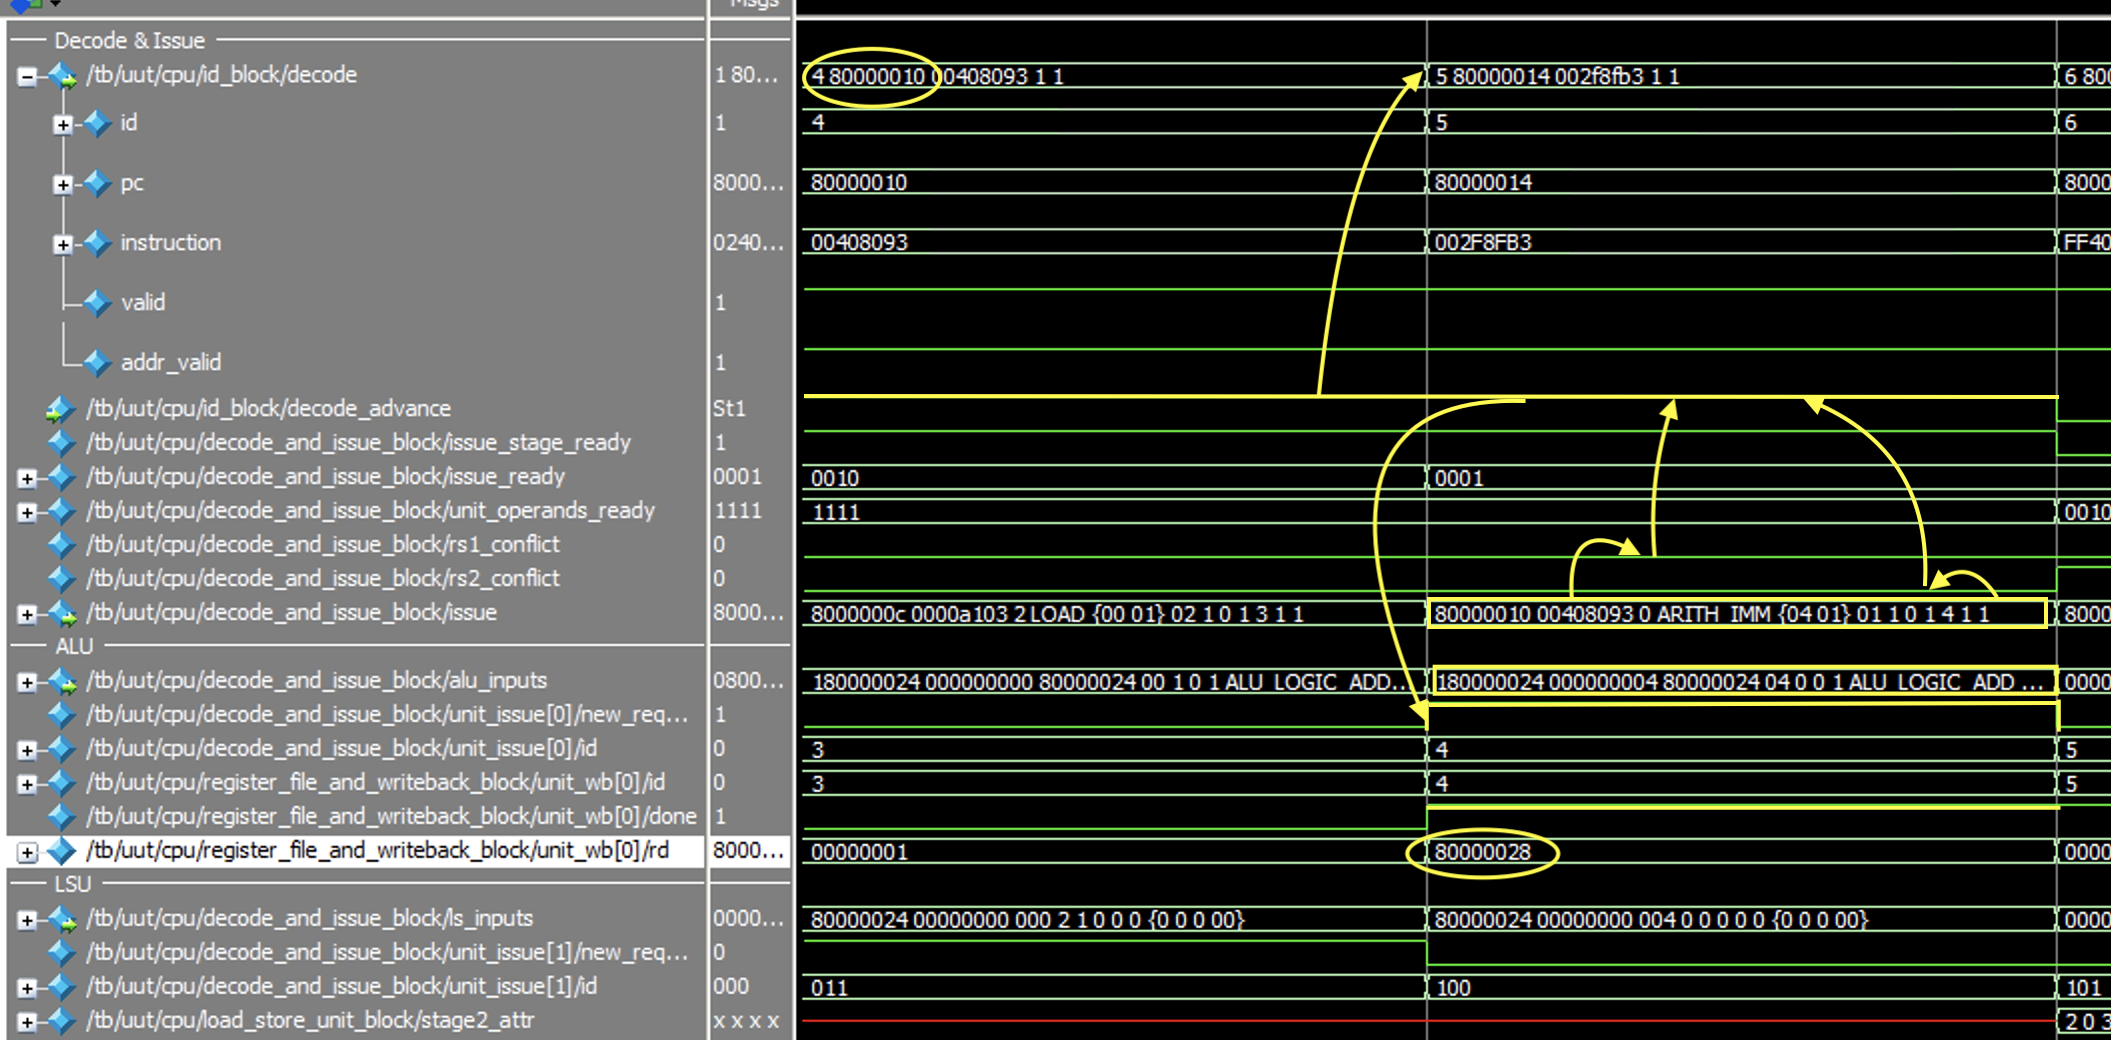
\includegraphics[width = \linewidth]{80000010_02.png}
	\caption{Временная диаграмма выполнения стадий декодирования, планирования на выполнение и выполнения команды с адресом 80000010}
	\label{80000010_02}
\end{figure}
\newpage
\section{Трасса выполнения программы}
В результате анализа диаграммы была заполнена трасса выполнения программы. Трасса выполнения показана на рисунке \ref{not_opt}

\begin{figure}[h!p]
	\centering
	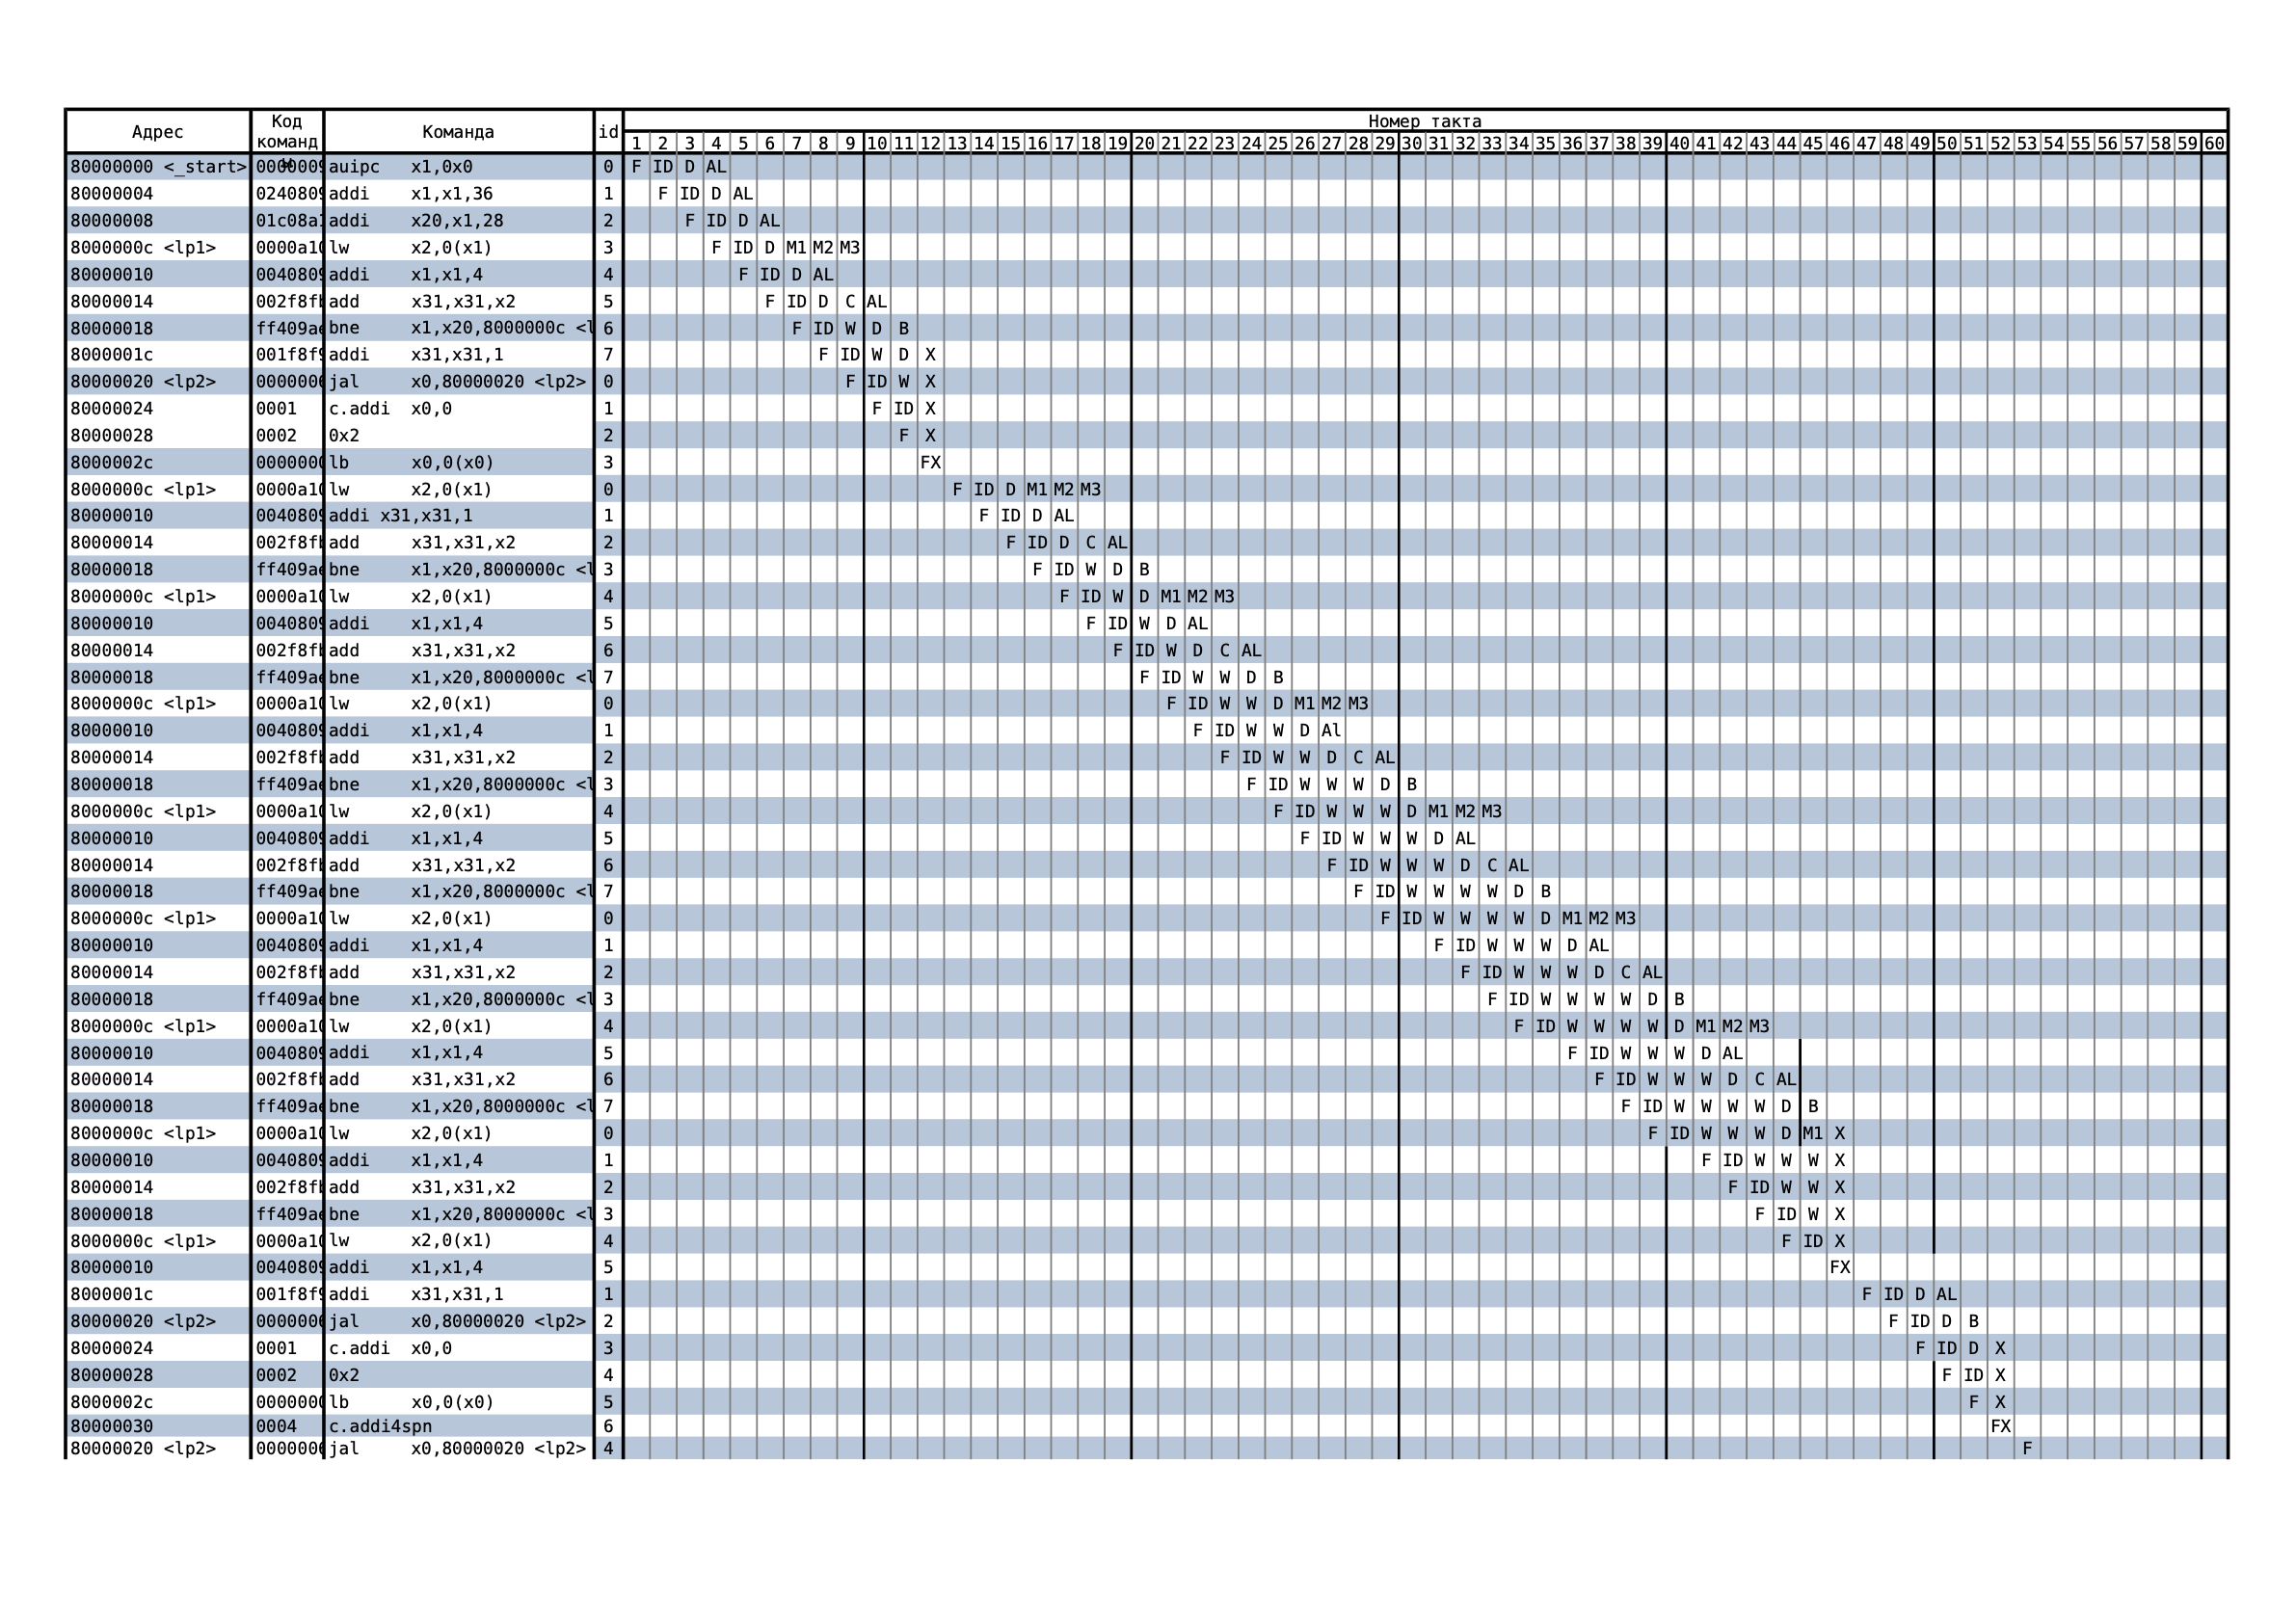
\includegraphics[width = \linewidth]{not_opt.png}
	\caption{Трасса выполнения программы}
	\label{not_opt}
\end{figure}

\section{Оптимизация программы}
Из анализа программы видно, что отсутствует возможность сократить время выполнения путем перестановки команд для ликвидации конфликтов и ожиданий декодера.

\section*{Вывод}
\addcontentsline{toc}{section}{Вывод}
Выполняемая программа имеет оптимальный порядок команд и не нуждается в оптимизации. 

\chapter*{Заключение}
\addcontentsline{toc}{chapter}{Заключение}
В данной лабораторной работе было проведено ознакомление с архитектурой ядра Taiga, а именно с порядком работы вычислительного конвейера: изучены команды RV32I, рассмотрены действия, выполняемые на каждой стадии конвейера, и данные, передаваемые между ними.
После ознакомления с теоретической стороной вопроса, был выполнен разбор этапов выполнения программы на симуляции процессора с набором инструкций RV32I. После ее анализа были сделаны выводы, что оптимизация не требуется.
В итоге, теоретические знания о порядке исполнения программ на процессорах с RISC архитектурой были закреплены на практике.
Таким образом все поставленные задачи решены, основная цель работы достигнута.

\end{document}